\section{Suchverfahren für Farbschemata}
\label{sec:farbschema}

In diesem Abschnitt wird eine Methode zur Lösung des Teilproblems $f_{scheme}: FGs \to P$ vorgeschlagen. Hierbei werden Farben aus $P$ für die Funktionsgruppen eines Layouts festgelegt, wodurch die Farbgestaltung der Webseite definiert wird. Zur Veranschaulichung wird ein exemplarisches Layout einer Webseite für Musikstreaming verwendet. Es enthält die in \autoref{sec:architektur} festgelegten Funktionsgruppen $FGs = $ \{Primär, Sekundär, Akzent, Interaktion, Text (neutral), Hintergrund (neutral)\}. \autoref{fig:fgs} hebt die Funktionsgruppen des Layouts separat hervor.

\begin{figure}[h]
\centering
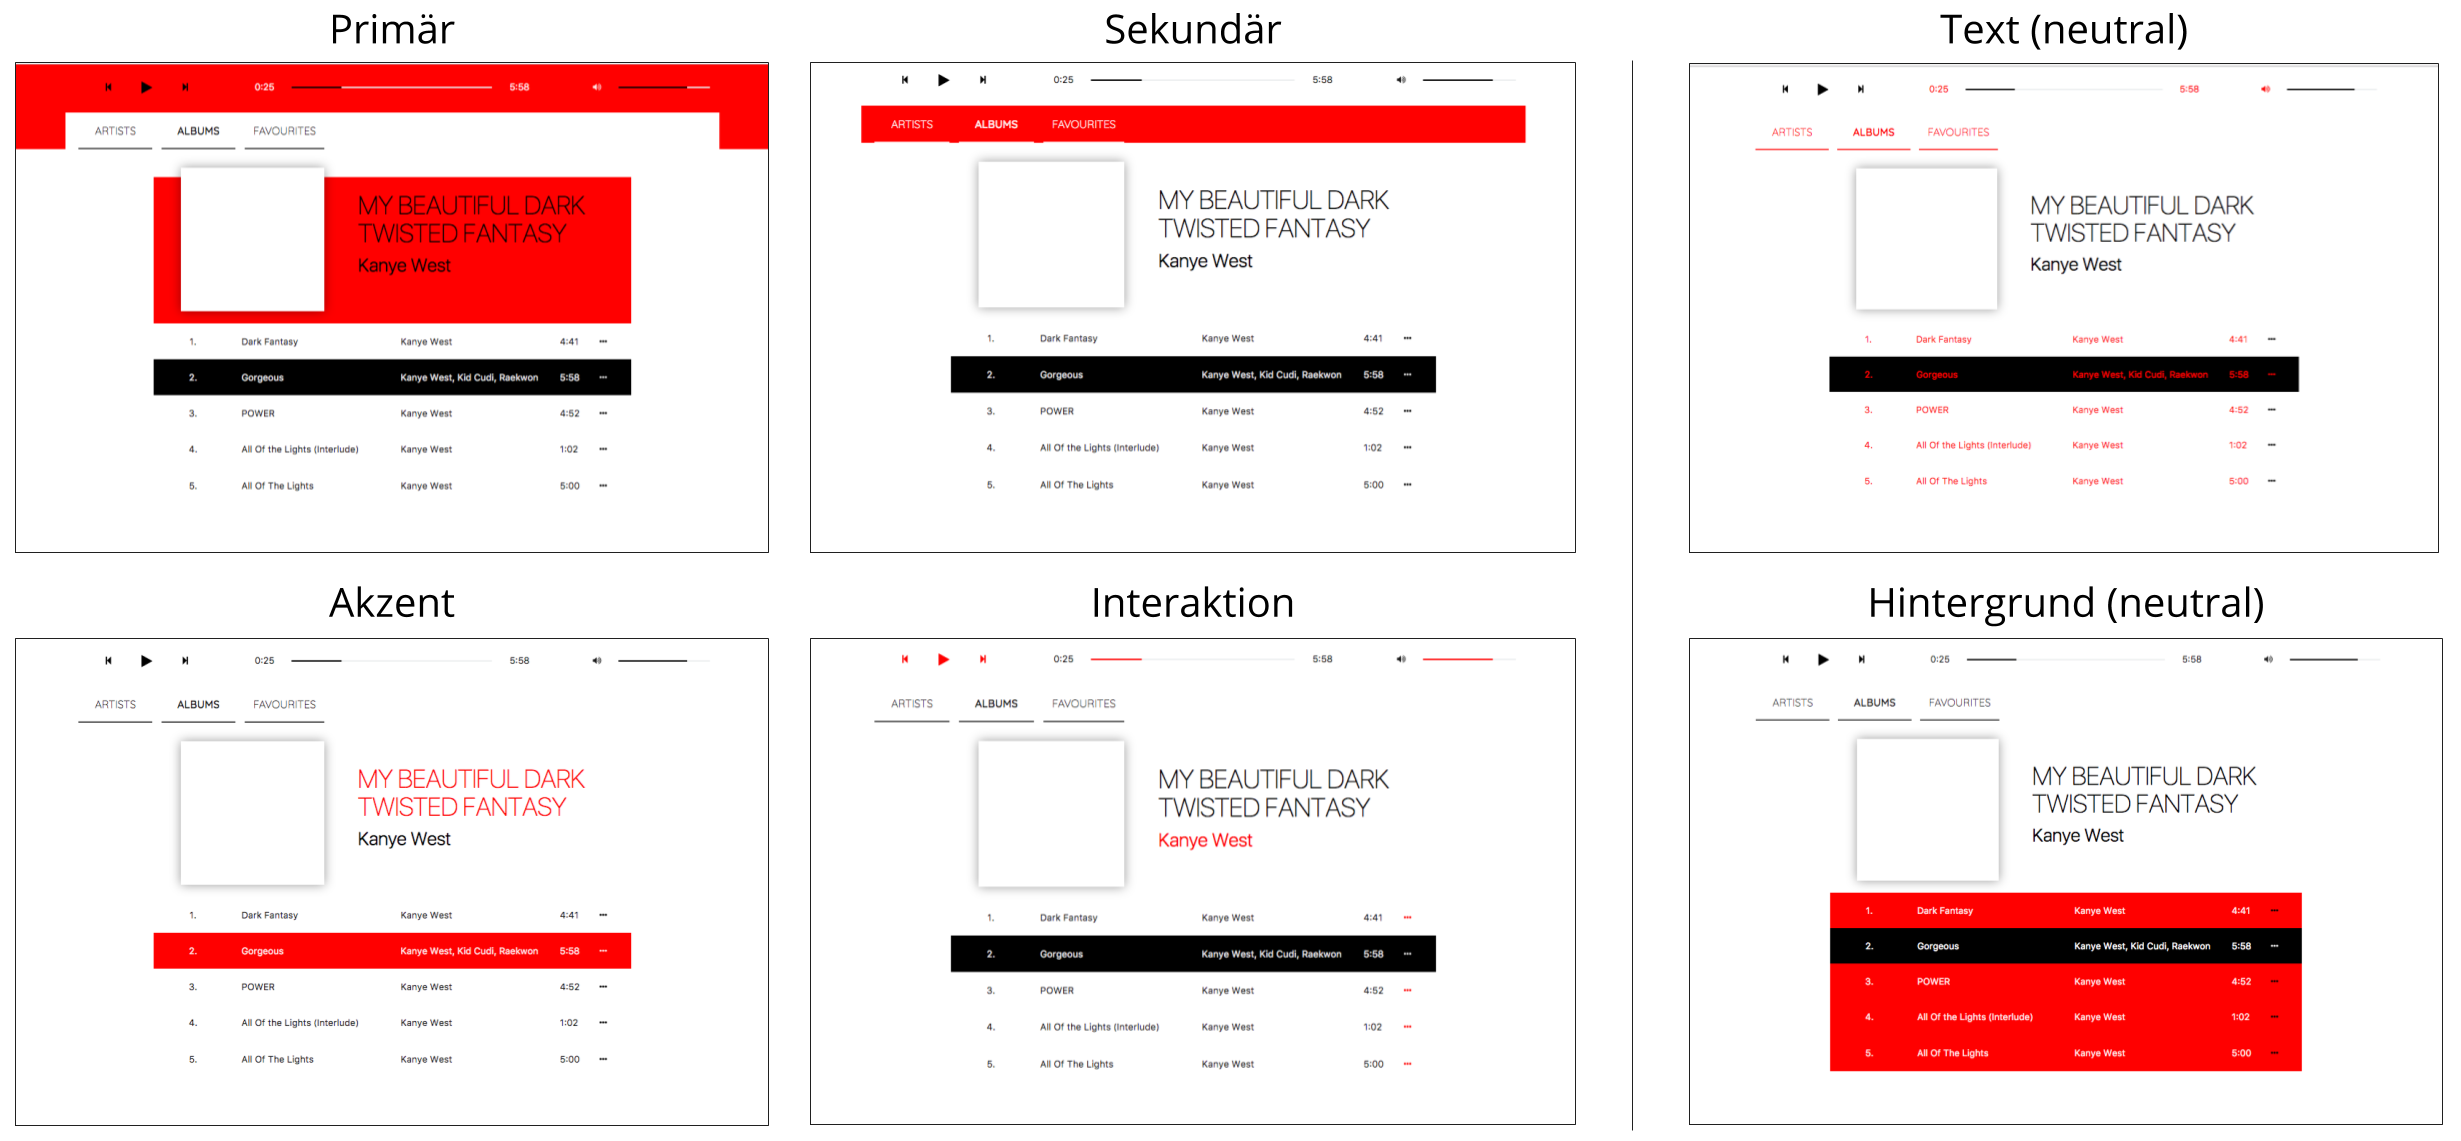
\includegraphics[width=0.95\textwidth]{img/fgs.png}
\caption{Funktionsgruppen des exemplarischen Layouts einer  Webseite für Musikstreaming. Alle Oberflächenkomponenten, die zur der jeweiligen Funktionsgruppe gehören, sind rot hervorgehoben.}
\label{fig:fgs}
\end{figure}

Für das Suchverfahren wurden Factor Graphs modelliert. Diese Methode wurde bereits erfolgreich in der Arbeit von \citet{magazines} zur Ermittlung der Farben von Flächen in Mustern eingesetzt. Ein Factor Graph ermöglicht die Beschreibung eines Constraint Graphen. Dieser repräsentiert die Aufspaltung einer komplexen Wahrscheinlichkeitsverteilung über mehrere Variablen durch deren Zerlegung in Teilfunktionen auf einer Teilmenge der Variablen. Zur Implementierung des Graphen sowie zur Inferenz möglicher Lösungen wird die Bibliothek \emph{Dimple}\footnote{\url{http://dimple.probprog.org/}} in der Programmiersprache Java verwendet.

Der Constraint-Graph besteht aus Knoten $V$ und Kanten $E$. Knoten beschreiben Variablen, für die Werte gesucht werden. In diesem Falle gilt $V = FGs\; \backslash$ \{Text (neutral)\}. Die Gruppe \{Text (neutral)\} wird ausgelassen, da entsprechend der Erläuterungen in \autoref{sec:architektur} die Entscheidung über die jeweilige Textfarbe der Blockelemente auf Layout-Ebene  getroffen wird und nicht Teil des Suchverfahrens ist. Der Wertebereich der Variablen für die FGs \{Primär, Sekundär, Akzent, Interaktion\} ist eine finite Domain $dom = \{d_1, ..., d_{n}\}$. Die Elemente in $dom$ korrespondieren mit Farbwerten in $P = \{c_1, .., c_n\}$ und stellen einen eigenen Datentyp dar. Die Attribute der $d \in dom$ lauten:

\begin{itemize}
	\item \textbf{$h$, $s$, $i$:} Der Farbwert im HSI Raum.
	\item \textbf{$r$, $g$, $b$:} Der Farbwert im RGB Raum. Wird für die Berechnung des Kontrastverhältnisses $L_c()$ benötigt.
	\item \textbf{Gewicht $weight$:} Relatives Gewicht des Segments in der hierarchischen Farbpalette. Hierzu werden die Gewichte (entsprechend \autoref{eq:weight}) aller Samples des Segments addiert und durch das Gewicht des gesamten Histogramms dividiert.
	\item \textbf{Hue-Group $hg$:} Index der Hue-Group der Farbe.
	\item \textbf{Größe der Hue-Group} $hg_\text{size}$: Relativer Anteil der Farben in $P$, die $\in hg$ sind.
\end{itemize}

Für die Funktionsgruppe \{Hintergrund (neutral)\} wird der Suchraum auf $weiss$ und $schwarz$ beschränkt.

Die Kanten $E$ entsprechen Constraints zwischen den Knoten. Es wird in Hard und Soft Constraints unterschieden \citep{patterns}. Hard Constraints beschreiben Einschränkungen, die bei der Lösung des Systems nicht verletzt werden dürfen. Soft Constraints beschreiben eine Gewichtung der möglichen Werte einer Variable in Form einer Bewertungsfunktion $score() \to [0, 1]$, wobei 1 für eine hohe und 0 für eine niedrige Bewertung steht. So sind Eigenschaften einer Farbe beschreibbar, die in Bezug auf eine Funktionsgruppe erwünscht sind (z.B. eine möglichst hohe Sättigung der Farbe für die Akzentgruppe).

In \autoref{sec:farbschemata} wurde der Typ eines Farbschemas daran unterschieden, wie viele verschiedene Farbtöne enthalten sind. Ein \emph{monochromes} Farbschema enthält einen Farbton, ein \emph{duales} zwei und ein \emph{triadisches} Farbschema drei verschiedene Farbtöne. Der ACoPa-Algorithmus ermittelt die Anzahl verschiedener Farbtöne eines Bildes, wodurch ebenfalls der Typ einer Farbpalette durch Analyse der Anzahl enthaltener Hue-Groups $\#HGs(P)$ feststellbar ist. Dementsprechend führt eine Farbpalette mit $\#HGs(P) = 1$ zu einem monochromen Farbschema, eine Farbpalette mit $\#HGs(P) = 2$ zu einem dualen und mit $\#HGs(P) \geq 3$ zu einem triadischen Farbschema. Auf diese Art und Weise spiegelt sich die wahrgenommene \glqq{}Buntheit\grqq{} einer Bildvorlage (im Sinne der Anzahl enthaltener Farbtöne) in einer entsprechend bunten Weboberfläche wieder, und umgekehrt. Farbpaletten mit mehr als drei verschiedenen Farbtönen werden auf ein triadisches Farbschema reduziert, da entsprechend \autoref{sec:farbschemata} die Verwendung von mehr Farbtönen nicht sinnvoll für die Benutzerführung ist.

Im Folgenden wird für jeden Typ ein separater Factor Graph entworfen. Die Ergebnisse werden anhand des prototypischen Layouts aus \autoref{fig:fgs} veranschaulicht.

\subsection{Suchverfahren für triadische Farbschemata}

\autoref{fig:scheme_triadic} visualisiert den Factor Graph für das triadische Farbschema (Fall: $\#HGs(P) \geq 3$). Die Kreise repräsentieren die Variablen. Quadrate repräsentieren Constraints, die sich auf die Variablen beziehen, zu denen Verbindungen eingezeichnet sind. Hard Constraints sind rot dargestellt, Soft Constraints gelb. Im Folgenden werden die Constraints erläutert.

Hard Constraints:
\begin{itemize}
	\item \textbf{cont:} Das Kontrastverhältnis $L_c$ muss mindestens 3.0 betragen, was den in \autoref{sec:lesbarkeit}) erläuterten Minimalvoraussetzungen für Textlesbarkeit  entspricht.\\
		$L_c(\text{value}(V_\text{Primär}), \text{value}(V_\text{Akzent})) \geq 3.0$\\
		$L_c(\text{value}(V_\text{Primär}), \text{value}(V_\text{Akzent})) \geq 3.0$
	\item \textbf{diff HG:} Die Hue-Groups müssen sich unterscheiden. \\ $\text{value}(V_\text{Primär}).hg \neq \text{value}(V_\text{Akzent}).hg \neq \text{value}(V_\text{Interaktion}).hg$
	\item \textbf{se:} Primär- und Sekundärfarbe müssen der gleichen Hue-Group angehören.\\
		$\text{value}(V_\text{Primär}).hg = \text{value}(V_\text{Sekundär}).hg$
\end{itemize}

Soft Constraints:
\begin{itemize}
	\item \textbf{pr:} Die Primärfarbe soll eine möglichst hohe Gewichtung im Histogramm besitzen, was auf eine hohe visuelle Relevanz in der Bildvorlage schließen lässt.\\
		$\forall d \in dom: score(d) = d.weight$
	\item \textbf{se:} Die Sekundärfarbe soll eine Sättigungsdifferenz zur Primärfarbe aufweisen.\\
		$\forall d \in dom: score(d) = | \text{value}(V_\text{Primär}).s - d.s |$
	\item \textbf{ak:} Die Akzentfarbe soll einer möglichst kleinen Hue-Group angehören, wodurch sie mit hoher Wahrscheinlichkeit ebenfalls einen Akzent in der Bildvorlage darstellt. Außerdem soll die Sättigung möglichst hoch sein.\\
		$\forall d \in dom: score(d) = (1 - d.hg_\text{size})\ d.s$
	\item \textbf{in:} Die Interaktionsfarbe soll eine möglichst hohe Sättigung besitzen.\\
		$\forall d \in dom: score(d) = d.s$
	\item \textbf{hr:} Für die Hintergrundfarbe (neutral) werden die globalen Farbinformationen verwendet. Ist die durschnittliche Luminanz der Farbwerte der Bildvorlage $> 0.2$, wird $weiss$ verwendet, sonst $schwarz$.
\end{itemize}

\begin{equation*}
  \text{value}(V_\text{Hintergrund}) =
  \begin{cases}
  	weiss, \; \text{wenn} \frac{\sum_{(x, y) \in I} L(\text{color}(x, y))}{|I|} > 0.2\\
  	schwarz, \; sonst
  \end{cases}
\end{equation*}

\begin{figure}[h]
\centering
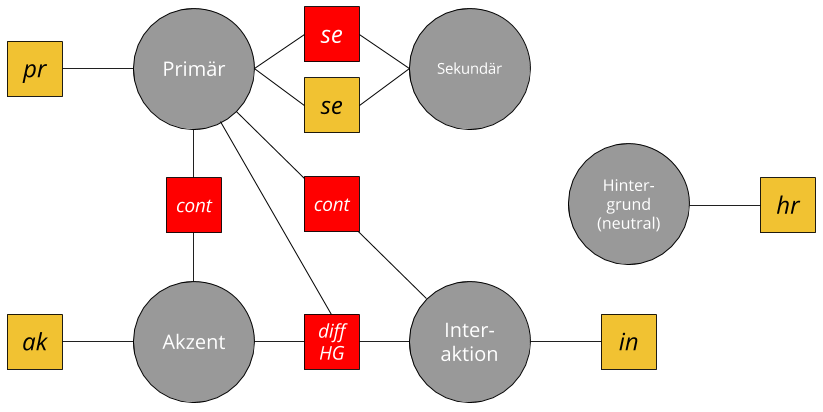
\includegraphics[width=0.75\textwidth]{img/scheme_triadic.png}
\caption{Factor Graph zur Bildung triadischer Farbschemata. Die Variablen werden rund, Hard Constraints rot und Soft Constraints gelb dargestellt.}
\label{fig:scheme_triadic}
\end{figure}

\autoref{fig:results_triadic} veranschaulicht die Ergebnisse des Suchverfahrens anhand der exemplarischen Weboberfläche für Musikstreaming. Dabei zeigt (b) jeweils die hierarchische Farbpalette mit den Funktionsgruppen, die durch Inferenz auf dem Factor Graph von Dimple zugeordnet wurden. \emph{Pr} steht für Primär, \emph{Se} für Sekundär, \emph{Ak} für Akzent, \emph{In} für Interaktion und \emph{Hi} für Hintergrund (neutral). Die Farbe für letztere Funktionsgruppe ist abgesetzt dargestellt, da sie nicht Teil der hierarchischen Farbpalette ist. Der Gradient wird via CSS beschrieben und verläuft von der Primär- zur Akzentfarbe mit einem Alpha-Wert von 0.8.

\begin{itemize}
	\item \textbf{Ergebnis Nr. 1:} Erwartungsgemäße Färbung. Die Wahl der Primärfarbe unterstützt die Lesbarkeit.
	\item \textbf{Ergebnis Nr. 2:} Blau wurde aufgrund des hohen visuellen Gewichts in der Bildvorlage als Primärfarbe selektiert. Da sich keine weitere Farbe in der selben Hue-Group befindet, wird die Sekundärfarbe auf den selben Farbwert abgebildet.
	 \item \textbf{Ergebnis Nr. 3:} Obwohl Gelb visuell  als Akzent in der Bildvorlage hervortritt, wird es als Interaktions- und nicht als Akzentfarbe bestimmt. Grund ist deren Mitgliedschaft in der Hue-Group mit den Brauntönen, wodurch das Kriterium einer möglichst kleinen Hue-Group nicht erfüllt wird. Bei der Wahl der konkreten Helligkeitsstufe ist ein ansprechender Kompromiss zwischen Buntheit und Textlesbarkeit gelungen.
	 \item \textbf{Ergebnis Nr. 4:} Fall mit $\#HGs(P) > 3$. Trotz der vergleichsweise hohen Anzahl möglicher Farben wird die Primärfarbe erwartungsgemäß zugeordnet. Die Interaktionsfarbe wird zu Gunsten des Lesbarkeit auf eine Farbe mit geringem visuellen Effekt in der Bildvorlage abgebildet (die Lippen der Figur).
\end{itemize}

\subsection{Suchverfahren für duale Farbschemata}

\autoref{fig:scheme_dual} visualisiert den Factor Graph für das duale Farbschema (Fall: $\#HGs(P) = 2$). Im Gegensatz zum triadischen Farbschema wird die Wahl von Farbwerten mit unterschiedlichen Hue-Groups nur noch für die Primär- und Akzentfarbe erzwungen. Stattdessen verhindert der neue Hard Constraint \emph{diff var} die Wahl gleicher Farbwerte von Akzent-, Interaktions- und Sekundärfarbe.
 
 \begin{itemize}
	\item \textbf{Ergebnis Nr. 1:} Erwartungsgemäße Färbung.
	\item \textbf{Ergebnis Nr. 2:} Der violette Farbton wird zur Akzentfarbe, obwohl er zur größten Hue-Group gehört. Dies ist dem Umstand geschuldet, dass Dunkelblau als bester Kompromiss zwischen Textlesbarkeit und visuellem Gewicht zur Primärfarbe wird, Akzent- und Primärfarbe jedoch Teil unterschiedlicher Hue-Groups sein müssen. Primär- und Sekundärfarbe fallen zusammen, da Türkis zur Interaktionsfarbe gewählt wird und somit in der Hue-Group der Primärfarbe kein anderer Farbton mehr zur Auswahl steht. Aufgrund der durchschnittlichen Luminanz $\leq 2.0$ wird $schwarz$ als Hintergrund (neutral) festgelegt.
\end{itemize}
 
\begin{figure}[h]
\centering
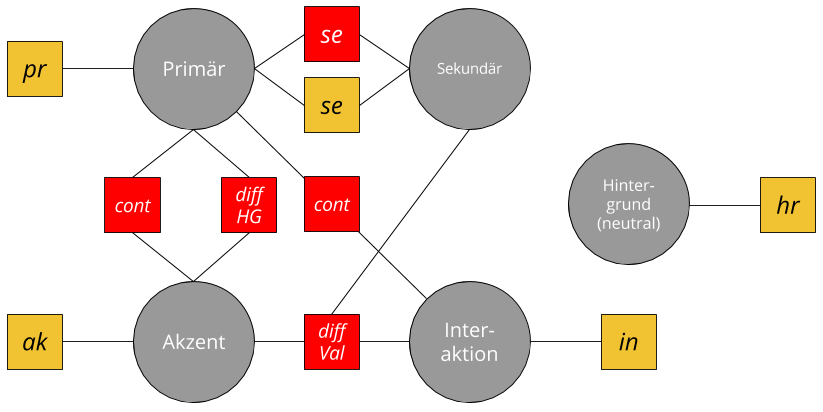
\includegraphics[width=0.75\textwidth]{img/scheme_dual.png}
\caption{Factor Graph zur Bildung dualer Farbschemata. Die Variablen werden rund, Hard Constraints rot und Soft Constraints gelb dargestellt.}
\label{fig:scheme_dual}
\end{figure}

\subsection{Suchverfahren für monochrome Farbschemata}

\autoref{fig:scheme_monochrom} visualisiert den Factor Graph für monochrome Farbschemata (Fall: $\#HGs(P) = 1$). Trotz der Orientierung der Farbgestaltung an der Bildvorlage darf die Benutzerführung nicht vernachlässigt werden. Aus diesem Grund wurde die Entscheidung getroffen, $P$ durch die Komplementärfarbe der gewählten Primärfarbe zu ergänzen und diese für die Akzent- und Interaktionsfarbe festzulegen. \autoref{fig:scheme_monochrom} zeigt den Factor Graph für monochrome Farbschemata, wobei nur die Primär- und Sekundärfarbe entschieden werden. Daraufhin wird der Farbton der Komplementärfarbe durch $h_\text{komplementär} = (\text{value}(V_\text{Primär}).h + 180.0) \mod 360.0$ errechnet. Abschließend wird die I-Komponente der Komplementärfarbe so lange verschoben, bis ein ausreichender Luminanzkontrast zur Primärfarbe erreicht wurde. \autoref{fig:results_monochrom} veranschaulicht das Ergebnis anhand einer Bildvorlage mit nur einem einzigen dominierenden Farbton.

\begin{figure}[h]
\centering
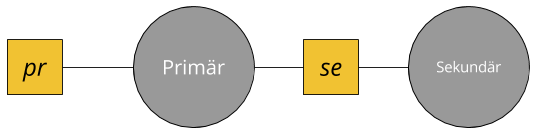
\includegraphics[width=0.75\textwidth]{img/scheme_monochrom.png}
\caption{Factor Graph zur Bildung monochromer Farbschemata. Die Variablen werden rund und Soft Constraints gelb dargestellt.}
\label{fig:scheme_monochrom}
\end{figure}

\begin{figure}[h]
\centering
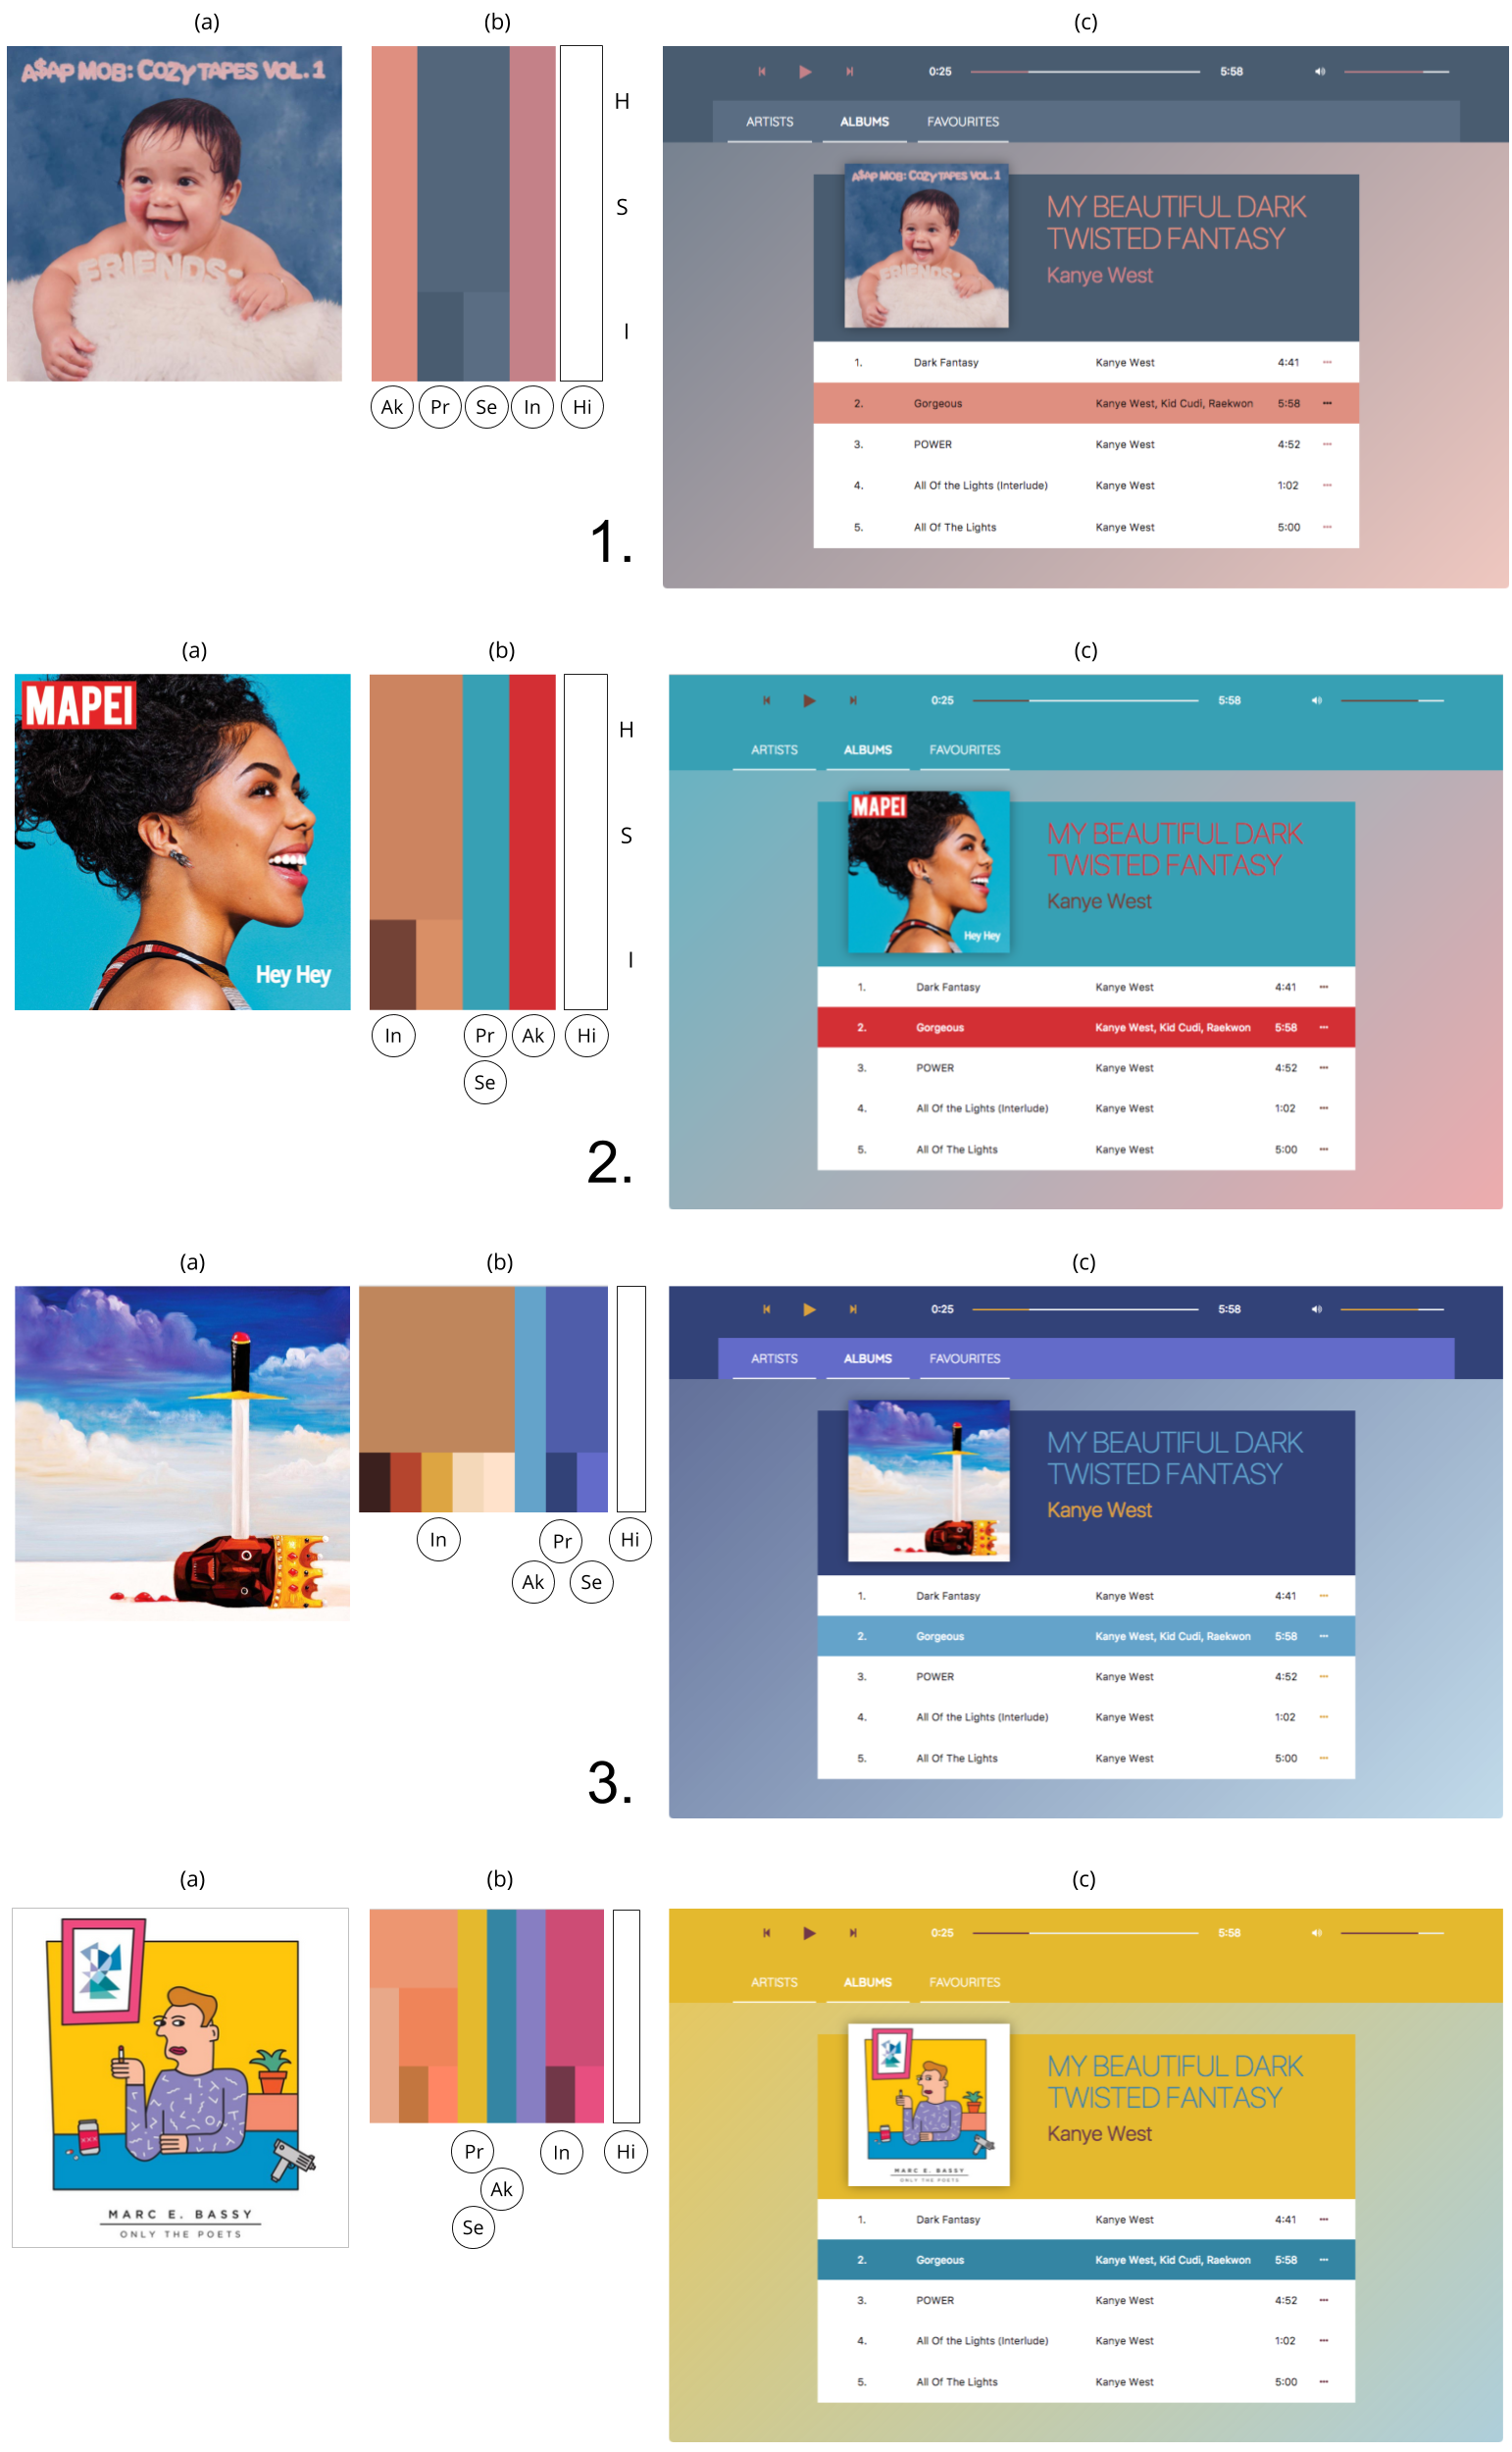
\includegraphics[width=0.92\textwidth]{img/results_triadic.png}
\caption{Ergebnis der automatisierten Farbgestaltung (triadisches Farbschema). (a) Bildvorlage. (b) Hierarchische Farbpalette mit Zuordnung der Funktionsgruppen. (c) Färbungsergebnis des exemplarischen Layouts aus \autoref{fig:fgs}.}
\label{fig:results_triadic}
\end{figure}

\begin{figure}[h]
\centering
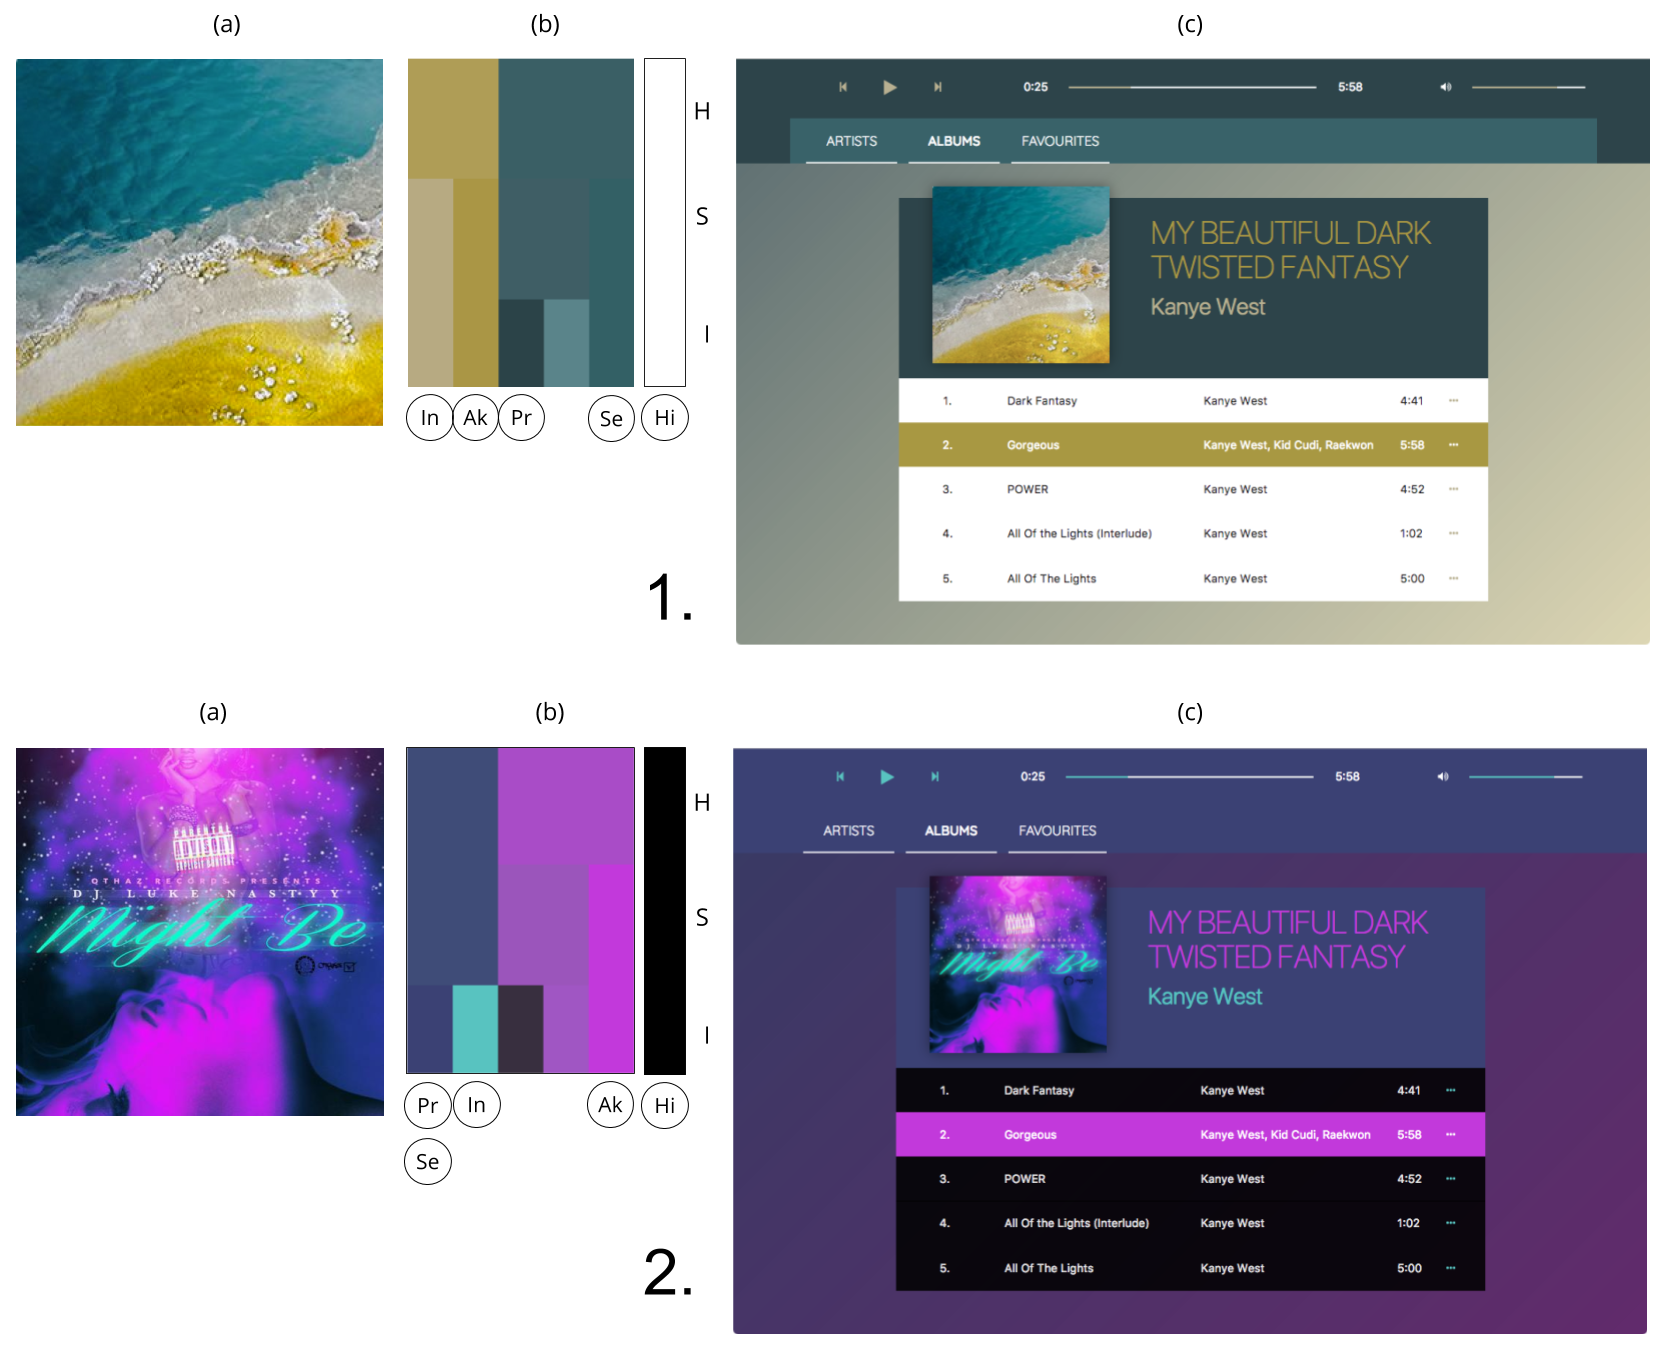
\includegraphics[width=0.92\textwidth]{img/results_dual.png}
\caption{Ergebnis der automatisierten Farbgestaltung (duales Farbschema). (a) Bildvorlage. (b) Hierarchische Farbpalette mit Zuordnung der Funktionsgruppen. (c) Färbungsergebnis des exemplarischen Layouts aus \autoref{fig:fgs}.}
\label{fig:results_dual}
\end{figure}

\begin{figure}[h]
\centering
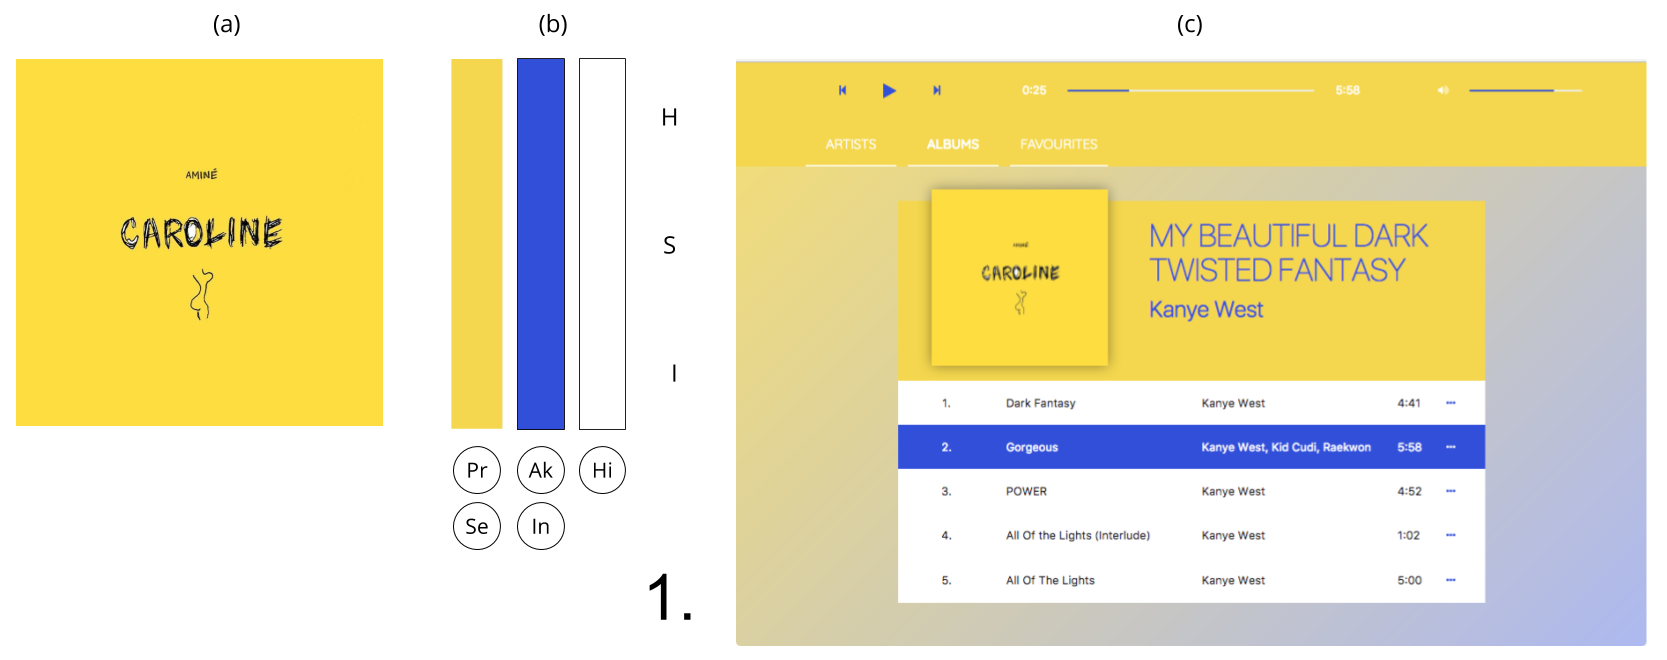
\includegraphics[width=0.92\textwidth]{img/results_monochrom.png}
\caption{Ergebnis der automatisierten Farbgestaltung (duales Farbschema). (a) Bildvorlage. (b) Hierarchische Farbpalette mit Zuordnung der Funktionsgruppen.  Die blaue Farbe wurde komplementär zur Primärfarbe berechnet. (c) Färbungsergebnis des exemplarischen Layouts aus \autoref{fig:fgs}.}
\label{fig:results_monochrom}
\end{figure}

